% 图 44.4 —— 由 `checks/emit_hand.py` 自动拼出（probe 精测 + prims2 图元分解）
%%
% ⚠ 这是**稿子不是成品**：跑 `checks/checkhand.py 44.4` 看指标 + 看叠合图。
%%
%% ⚠ 待核：
%   · 本图 probe 报出阴影族 1 个 —— **本脚本不生成阴影**（要照原书手写）；prims2 的 strokes 里可能含阴影线，核对时留意别画重
%   · 可疑字形 1 项（空心圈 ⊙ 常被认成字母 o）—— 见文件末
%%
\documentclass[12pt]{standalone}
\usepackage{fontspec}
\setsansfont{Arial}
\newfontfamily\mfallback{DejaVu Sans}
\usepackage{tikz}
\begin{document}
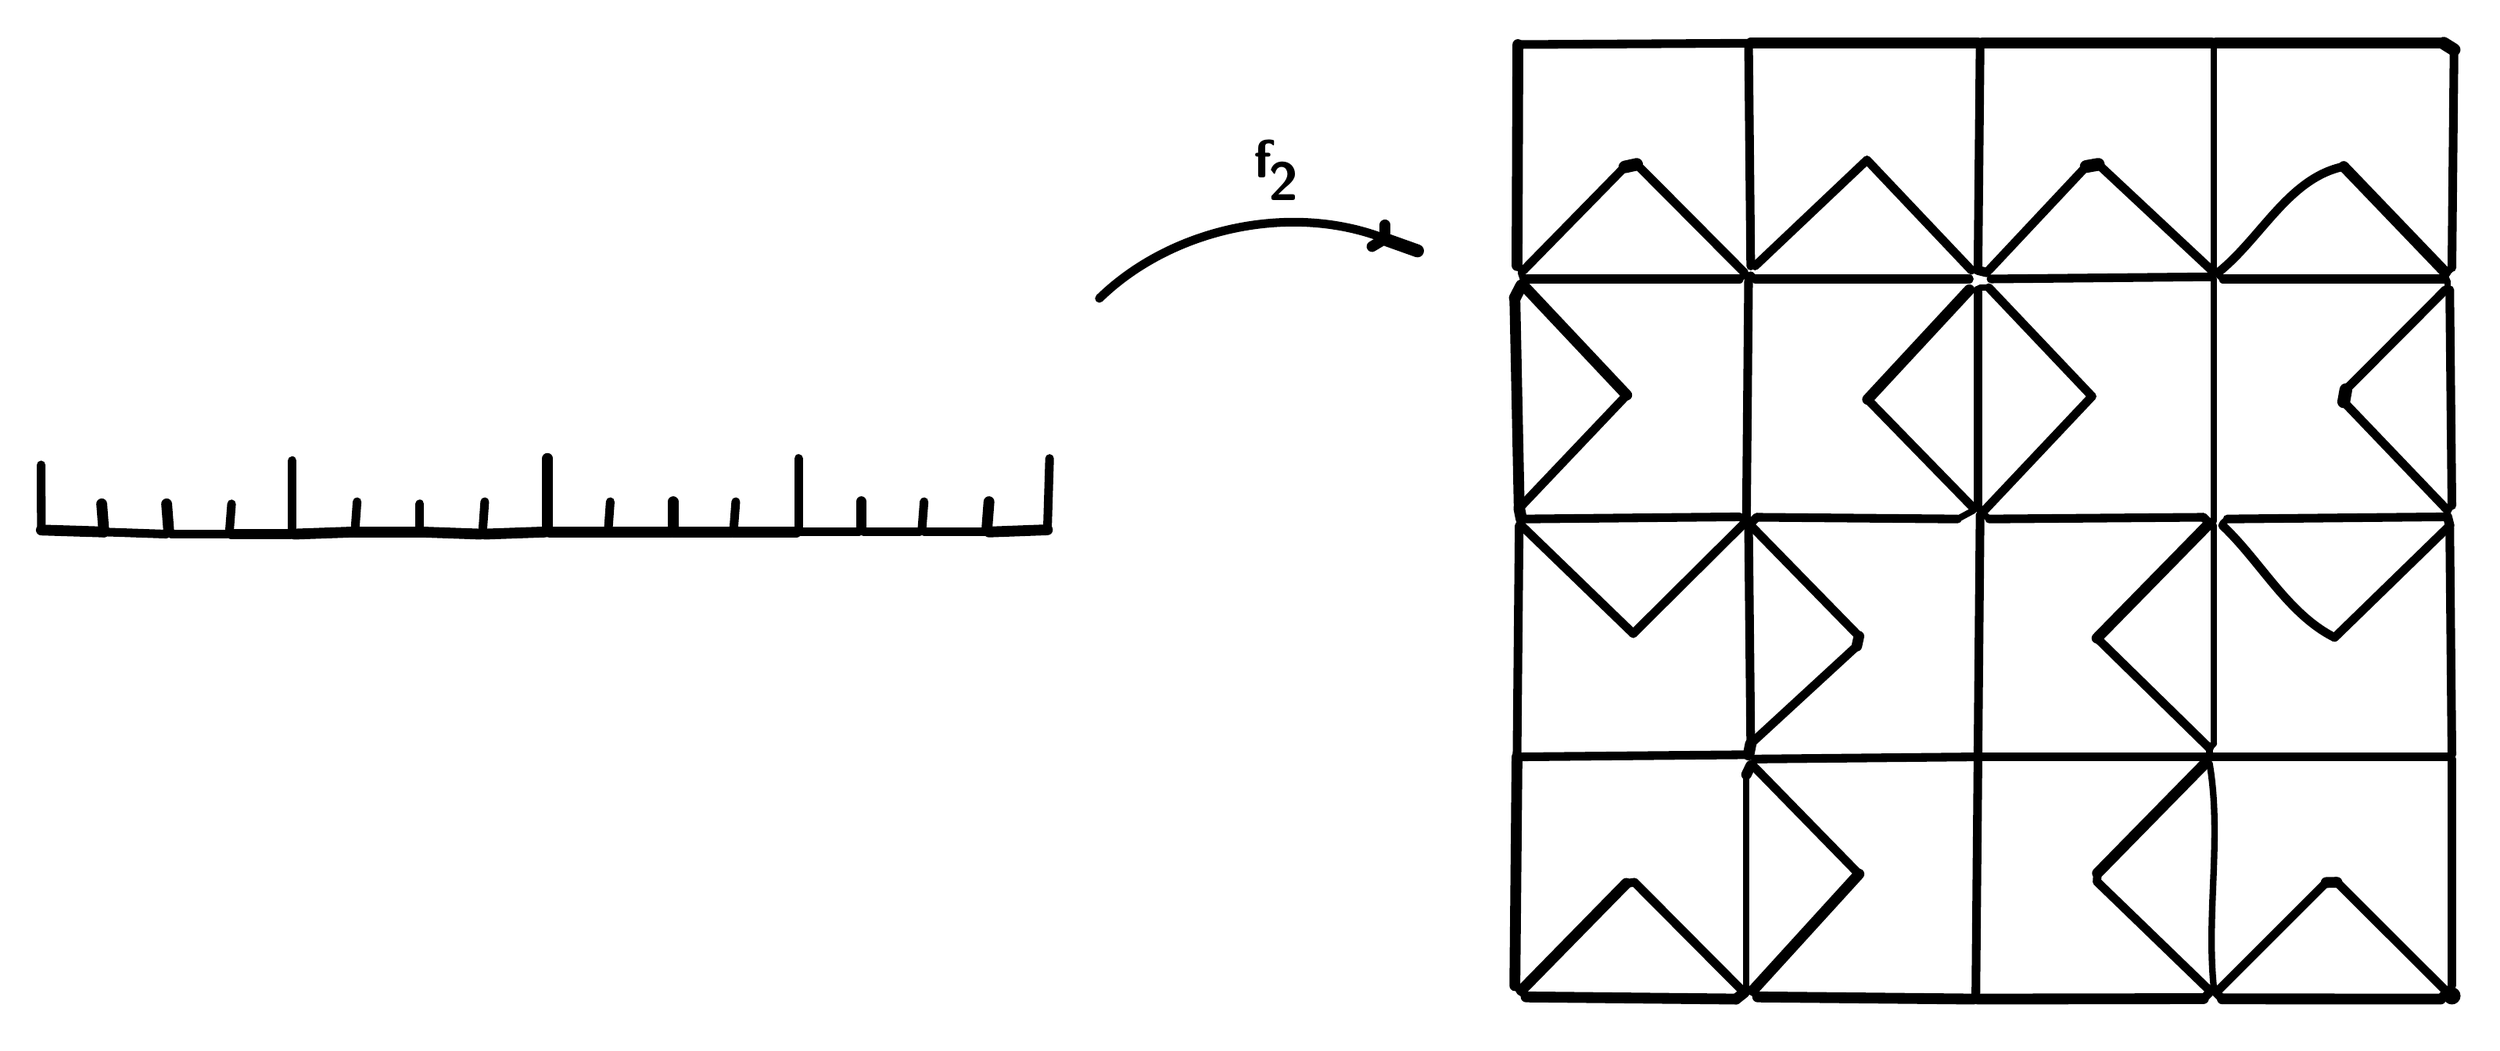
\begin{tikzpicture}[x=1pt, y=-1pt, line width=5.0pt, line cap=round, line join=round]

  %% ════ 填充区（prims2 的 fills）════

  %% ════ 直线段（prims2 的 strokes）════
  \draw[line width=5.0pt] (624.0,104.0) -- (629.0,101.0);
  \draw[line width=4.0pt] (692.0,233.0) -- (691.0,340.0);
  \draw[line width=5.0pt] (904.0,452.0) -- (1008.2,451.8);
  \draw[line width=4.0pt] (1008.2,451.8) -- (1011.0,449.0);
  \draw[line width=4.0pt] (904.0,124.0) -- (904.0,225.0);
  \draw[line width=4.0pt] (96.0,236.0) -- (97.0,223.0);
  \draw[line width=4.3pt] (1122.0,233.0) -- (1121.0,229.0);
  \draw[line width=4.0pt] (798.0,11.0) -- (799.0,113.0);
  \draw[line width=4.0pt] (359.0,202.0) -- (359.0,235.0);
  \draw[line width=3.0pt] (905.0,123.0) -- (908.0,123.0);
  \draw[line width=3.0pt] (1011.0,339.0) -- (1011.0,336.0);
  \draw[line width=5.0pt] (97.0,237.0) -- (124.0,237.0);
  \draw[line width=5.0pt] (1009.0,343.0) -- (959.2,393.8);
  \draw[line width=3.9pt] (959.2,393.8) -- (959.0,397.7);
  \draw[line width=4.0pt] (959.0,397.7) -- (1011.0,448.0);
  \draw[line width=5.0pt] (242.0,236.0) -- (214.0,237.0);
  \draw[line width=4.0pt] (801.0,341.0) -- (903.0,340.0);
  \draw[line width=5.0pt] (630.0,99.0) -- (630.0,94.0);
  \draw[line width=5.0pt] (1012.0,10.0) -- (906.0,10.0);
  \draw[line width=3.0pt] (902.0,226.0) -- (894.6,230.0);
  \draw[line width=4.0pt] (894.6,230.0) -- (801.8,229.2);
  \draw[line width=4.0pt] (801.8,229.2) -- (799.0,232.0);
  \draw[line width=4.8pt] (799.0,344.0) -- (797.0,348.2);
  \draw[line width=3.0pt] (797.0,348.2) -- (797.0,448.0);
  \draw[line width=4.0pt] (1120.0,119.0) -- (1017.2,119.0);
  \draw[line width=3.0pt] (1017.2,119.0) -- (1015.0,117.0);
  \draw[line width=5.0pt] (244.0,236.0) -- (271.0,236.0);
  \draw[line width=4.0pt] (1123.0,339.0) -- (1122.0,234.0);
  \draw[line width=3.0pt] (800.0,449.0) -- (802.2,451.0);
  \draw[line width=5.0pt] (802.2,451.0) -- (902.0,452.0);
  \draw[line width=4.0pt] (904.0,114.0) -- (905.0,11.0);
  \draw[line width=4.0pt] (1012.0,340.0) -- (1122.0,340.0);
  \draw[line width=3.0pt] (1121.0,116.0) -- (1123.0,113.8);
  \draw[line width=4.0pt] (1123.0,113.8) -- (1124.0,13.0);
  \draw[line width=5.9pt] (1124.0,13.0) -- (1119.2,10.0);
  \draw[line width=5.0pt] (1119.2,10.0) -- (1014.0,10.0);
  \draw[line width=4.0pt] (1121.0,226.0) -- (1073.0,175.8);
  \draw[line width=5.9pt] (1073.0,175.8) -- (1074.0,170.2);
  \draw[line width=4.0pt] (1074.0,170.2) -- (1120.0,124.0);
  \draw[line width=3.0pt] (1121.0,226.0) -- (1123.0,223.8);
  \draw[line width=4.0pt] (1123.0,223.8) -- (1122.0,124.0);
  \draw[line width=4.0pt] (799.0,333.0) -- (798.0,234.0);
  \draw[line width=4.0pt] (445.0,236.0) -- (417.0,236.0);
  \draw[line width=4.0pt] (272.0,222.0) -- (271.0,236.0);
  \draw[line width=3.0pt] (1121.0,448.0) -- (1123.0,445.8);
  \draw[line width=4.0pt] (1123.0,445.8) -- (1123.0,341.0);
  \draw[line width=4.0pt] (1120.0,449.0) -- (1117.8,452.0);
  \draw[line width=5.0pt] (1117.8,452.0) -- (1016.9,451.9);
  \draw[line width=4.0pt] (1016.9,451.9) -- (1014.0,449.0);
  \draw[line width=3.0pt] (796.0,117.0) -- (793.8,119.0);
  \draw[line width=4.0pt] (793.8,119.0) -- (695.0,119.0);
  \draw[line width=5.3pt] (692.0,225.0) -- (693.0,230.0);
  \draw[line width=5.0pt] (904.0,10.0) -- (799.0,10.0);
  \draw[line width=4.0pt] (903.0,451.0) -- (904.0,341.0);
  \draw[line width=3.0pt] (1121.0,120.0) -- (1121.0,123.0);
  \draw[line width=4.0pt] (693.0,224.0) -- (741.7,172.7);
  \draw[line width=5.0pt] (741.7,172.7) -- (694.0,122.0);
  \draw[line width=4.0pt] (909.0,123.0) -- (956.7,173.3);
  \draw[line width=4.0pt] (956.7,173.3) -- (907.0,226.0);
  \draw[line width=5.0pt] (301.0,236.0) -- (328.0,236.0);
  \draw[line width=4.0pt] (799.0,233.0) -- (849.0,284.2);
  \draw[line width=4.9pt] (849.0,284.2) -- (848.0,288.8);
  \draw[line width=4.0pt] (848.0,288.8) -- (800.0,333.0);
  \draw[line width=3.0pt] (1017.0,232.0) -- (1019.2,230.0);
  \draw[line width=4.0pt] (1019.2,230.0) -- (1120.0,229.0);
  \draw[line width=6.0pt] (631.0,101.0) -- (645.0,106.0);
  \draw[line width=5.5pt] (693.0,122.0) -- (690.0,127.8);
  \draw[line width=5.0pt] (690.0,127.8) -- (692.0,224.0);
  \draw[line width=5.3pt] (798.0,339.0) -- (799.0,334.0);
  \draw[line width=4.0pt] (798.0,339.0) -- (691.0,340.0);
  \draw[line width=5.0pt] (38.0,236.0) -- (37.0,223.0);
  \draw[line width=5.0pt] (38.0,236.0) -- (9.1,235.1);
  \draw[line width=4.0pt] (9.1,235.1) -- (9.0,205.0);
  \draw[line width=4.0pt] (38.0,236.0) -- (67.0,237.0);
  \draw[line width=4.0pt] (475.0,202.0) -- (474.0,235.0);
  \draw[line width=5.0pt] (474.0,235.0) -- (447.0,236.0);
  \draw[line width=5.0pt] (358.0,236.0) -- (329.0,236.0);
  \draw[line width=5.0pt] (243.0,235.0) -- (243.0,202.0);
  \draw[line width=5.0pt] (68.0,236.0) -- (67.0,223.0);
  \draw[line width=4.3pt] (908.0,116.0) -- (904.0,115.0);
  \draw[line width=4.0pt] (69.0,237.0) -- (95.0,237.0);
  \draw[line width=4.0pt] (905.0,228.0) -- (904.0,339.0);
  \draw[line width=4.0pt] (415.0,236.0) -- (389.0,236.0);
  \draw[line width=4.0pt] (798.0,118.0) -- (797.0,230.0);
  \draw[line width=4.0pt] (360.0,236.0) -- (387.0,236.0);
  \draw[line width=4.0pt] (1009.0,340.0) -- (905.0,340.0);
  \draw[line width=4.0pt] (909.0,115.0) -- (954.0,67.0);
  \draw[line width=5.9pt] (954.0,67.0) -- (959.6,66.0);
  \draw[line width=4.0pt] (959.6,66.0) -- (1012.0,115.0);
  \draw[line width=3.0pt] (1013.0,231.0) -- (1013.0,119.0);
  \draw[line width=4.0pt] (125.0,236.0) -- (125.0,203.0);
  \draw[line width=4.0pt] (900.0,119.0) -- (801.2,119.0);
  \draw[line width=3.0pt] (801.2,119.0) -- (799.0,117.0);
  \draw[line width=5.0pt] (388.0,222.0) -- (388.0,235.0);
  \draw[line width=5.0pt] (446.0,235.0) -- (447.0,222.0);
  \draw[line width=5.0pt] (271.0,236.0) -- (300.0,236.0);
  \draw[line width=3.0pt] (796.0,231.0) -- (793.8,229.0);
  \draw[line width=4.0pt] (793.8,229.0) -- (694.0,230.0);
  \draw[line width=5.0pt] (126.0,237.0) -- (154.0,236.0);
  \draw[line width=5.0pt] (691.0,340.0) -- (690.0,445.8);
  \draw[line width=3.0pt] (690.0,445.8) -- (692.0,448.0);
  \draw[line width=3.0pt] (907.0,228.0) -- (909.2,230.0);
  \draw[line width=4.0pt] (909.2,230.0) -- (1008.2,229.2);
  \draw[line width=4.0pt] (1008.2,229.2) -- (1011.0,232.0);
  \draw[line width=3.0pt] (1013.0,114.0) -- (1013.0,11.0);
  \draw[line width=3.4pt] (693.0,116.0) -- (694.0,119.0);
  \draw[line width=4.0pt] (902.0,225.0) -- (853.0,174.7);
  \draw[line width=5.0pt] (853.0,174.7) -- (900.0,124.0);
  \draw[line width=5.0pt] (693.0,448.0) -- (741.5,398.5);
  \draw[line width=4.0pt] (741.5,398.5) -- (745.3,398.0);
  \draw[line width=4.0pt] (745.3,398.0) -- (796.0,449.0);
  \draw[line width=4.0pt] (329.0,235.0) -- (330.0,222.0);
  \draw[line width=4.0pt] (154.0,236.0) -- (155.0,222.0);
  \draw[line width=5.0pt] (154.0,236.0) -- (184.0,236.0);
  \draw[line width=4.0pt] (184.0,223.0) -- (184.0,236.0);
  \draw[line width=4.0pt] (694.0,115.0) -- (740.8,67.2);
  \draw[line width=5.8pt] (740.8,67.2) -- (746.3,66.0);
  \draw[line width=4.0pt] (746.3,66.0) -- (796.0,116.0);
  \draw[line width=5.0pt] (301.0,222.0) -- (301.0,235.0);
  \draw[line width=5.0pt] (184.0,236.0) -- (212.0,237.0);
  \draw[line width=5.0pt] (1073.0,67.0) -- (1120.0,116.0);
  \draw[line width=4.0pt] (1012.0,118.0) -- (910.0,119.0);
  \draw[line width=4.0pt] (1015.0,448.0) -- (1064.9,398.1);
  \draw[line width=5.0pt] (1064.9,398.1) -- (1069.9,398.0);
  \draw[line width=4.0pt] (1069.9,398.0) -- (1120.0,448.0);
  \draw[line width=4.0pt] (416.0,235.0) -- (417.0,222.0);
  \draw[line width=4.0pt] (1011.0,336.0) -- (959.0,285.1);
  \draw[line width=5.0pt] (959.0,285.1) -- (1011.0,232.0);
  \draw[line width=3.0pt] (1011.0,336.0) -- (1013.0,333.8);
  \draw[line width=3.0pt] (1013.0,333.8) -- (1013.0,233.0);
  \draw[line width=4.0pt] (213.0,236.0) -- (214.0,222.0);
  \draw[line width=4.0pt] (693.0,233.0) -- (744.7,283.0);
  \draw[line width=4.0pt] (744.7,283.0) -- (796.0,232.0);
  \draw[line width=5.0pt] (800.0,448.0) -- (849.0,394.2);
  \draw[line width=4.0pt] (849.0,394.2) -- (800.0,344.0);
  \draw[line width=4.0pt] (1121.0,234.0) -- (1068.8,284.8);
  \draw[line width=4.0pt] (901.0,115.0) -- (852.7,64.0);
  \draw[line width=4.0pt] (852.7,64.0) -- (801.0,113.0);
  \draw[line width=3.0pt] (693.0,115.0) -- (691.0,112.8);
  \draw[line width=5.0pt] (691.0,112.8) -- (691.4,10.6);
  \draw[line width=4.0pt] (691.4,10.6) -- (797.0,10.0);
  \draw[line width=3.0pt] (693.0,449.0) -- (695.2,451.0);
  \draw[line width=5.0pt] (695.2,451.0) -- (792.2,452.0);
  \draw[line width=5.0pt] (792.2,452.0) -- (796.0,449.0);

  %% ════ 曲线（prims2 的 curves —— 三段式，坐标同为 (y,x)）════
  \draw[line width=4.0pt] (629.0,100.0) .. controls (585.9,83.7) and (531.2,95.6) .. (498.0,128.0);
  \draw[line width=3.0pt] (1011.0,343.0) .. controls (1016.8,376.7) and (1009.4,412.9) .. (1013.0,447.0);
  \draw[line width=4.0pt] (1015.0,116.0) .. controls (1035.0,100.0) and (1047.6,72.3) .. (1073.0,67.0);
  \draw[line width=4.0pt] (1068.8,284.8) .. controls (1047.2,274.0) and (1034.7,249.7) .. (1017.0,233.0);

  %% ════ 实心点 ════
  \fill (1123.0,450.5) circle (4.0);

  %% ════ 标签（probe 直接给的 \node 行）════
  %% ⚠ 全部补了 fill=white：文字在最上层，否则与曲线交叉干扰
     \node[anchor=center,inner sep=0pt,fill=white,font=\fontsize{27.1}{33.9}\selectfont] at (574.5,63.5) {\textsf{\textbf{\textit{f}}}};   % box(569,52,10,22)
     \node[anchor=center,inner sep=0pt,fill=white,font=\fontsize{25.7}{32.1}\selectfont] at (583.1,73.9) {\textsf{\textbf{2}}};   % box(576,65,13,17)

  % 钉死画布：否则超出的图元/控制点会把页面撑大，1:1 回比就失准
  \pgfresetboundingbox
  \path[use as bounding box] (0,0) rectangle (1135,466);
\end{tikzpicture}
\end{document}

% ⚠ 待核清单（probe 拿不准，人眼过一遍）：
%   · 未识别/跳过：⑤ 跳过/未识别的字形
